% !Mode::"TeX:UTF-8"
% !TExprogram  = xelatex
\documentclass[a4paper]{article}
\usepackage{amsmath}
\usepackage{amssymb}
\usepackage{ctex}
%\usepackage{braket}
%\usepackage[european]{circuitikz}
\usepackage{multirow}
\usepackage{float}
\usepackage{graphicx}
\usepackage{geometry}
\usepackage[version=4]{mhchem}
\usepackage{extarrows}
\usepackage{textcomp}
\usepackage{fontspec}
\usepackage{braket}
\usepackage{physics}
\usepackage{siunitx}
\sisetup{
	separate-uncertainty = true,
	inter-unit-product = \ensuremath{{}\cdot{}}
}
\geometry{left=2.5cm,right=2.5cm,bottom=2.5cm,top=2.5cm}
\title{近代物理实验报告10.5:原子力显微镜}
\author{林杨\quad 211840092\quad 物理学院}
\date{2024年5月17日}
\begin{document}
\maketitle

\tableofcontents

\newpage

\bibliographystyle{unsrt}
%--------main-body------------

\section{引言}
在当今的科学技术中,如何观察、测量、分析尺寸小于可见光波长的物体,是一个重要的研究方向。1982年,G. Binnig和H. Rohrer在IBM公司苏黎世实验室共同研制成功了第一台扫描隧道显微镜(Scanning Tunnelling Microscope, STM),使人们首次能够真正实时地观察到单个原子在物体表面的排列方式和表面电子行为有关的物理、化学性质。1986年,Binnig和Rohrer被授予诺贝尔物理学奖。但STM要求样品表面能够导电,从而使得STM只能直接观察导体和半导体的表面结构。为了克服STM的不足之处,Binnig、Quate和Gerber决定用微悬臂作为力信号的传播媒介,吧微悬臂放在样品和STM的针尖之间,于1986年推出了原子力显微镜(Atomic Force Microscope, AFM),AFM是通过针尖与被测样品之间微弱的相互作用力来获得物质表面形貌的信息,因此AFM除导电样品外,还能够观测非导电样品的表面结构,其应用领域更为广阔,除物理、化学、生物等领域外,AFM在微电子学、微机械学、新型材料、医学等领域有着广泛的应用。以STM和AFM为基础,衍生出了一系列的扫描探针显微镜(SPM),有激光力显微镜(LFM),磁力显微镜(MFM)等。扫描探针显微镜主要用于对物质表面在纳米级上进行成像和分析。

\section{实验目的}
\begin{enumerate}
\item 了解原子力显微镜的工作原理。
\item 初步掌握用原子力显微镜进行表面观测的方法。
\end{enumerate}

\section{实验仪器}
原子力显微镜:样品台、光源系统、测量控制系统。

\section{实验原理}
\subsection{AFM的工作原理和工作模式}
\subsubsection{AFM的工作原理}
在AFM中用一个安装在对微弱力极敏感的微悬臂上的极细探针代替STM中的金属极细探针,当探针与样品接触时,由于它们原子之间存在极微弱的作用力(吸引或排斥力),引起微悬臂偏转。扫描时控制这种作用力恒定,带针尖的微悬臂将对应于原子间作用力的等位面,在垂直于样品表面方向上起伏运动,因而会使反射光的位置改变而造成偏移量,通过光电检测系统对微悬臂的偏转进行扫描,测得微悬臂对应于扫描各点的位置变化,将信号放大与转换从而得到样品表面原子级的三维立体形貌图像。AFM的核心部件是力的传感器件,包括微悬臂(Cantilever)和固定于其一端的针尖。根据物理学原理,施加到微悬臂末端力的表达式为:
\begin{equation}
F = K\Delta Z\label{eq1}
\end{equation}
$\Delta Z$表示针尖相对于试样间的距离,K为微悬臂的弹性系数。力的变化均可以通过微悬臂被检测。
\subsubsection{AFM的关键部分}
AFM的关键部份是力敏感元件和力敏感检测装置。为了能够准确地反映出样品表面形貌,力传感器要满足以下几个要求:(1)在针尖与样品的接触过程中,为了不使针尖损坏样品,要求微悬臂有较低的力学弹性系数,即受到很小的力就能产生可检测的位移;(2)为了降低仪器对低频噪音的敏感性,并使其有较高的扫描速度,要求微悬臂有尽可能高的固有共振频率(一般为$\SI{200}{kHz}\sim\SI{300}{kHz}$);(3)因为微悬臂上的针尖与样品的摩擦力会引起微悬臂的横向弯曲,从而导致图像失真,这就要求微悬臂要有高的横向刚性,实际应用中将微悬臂制成V字形就可提高其横向刚性;(4)如果采用隧道电流方式来检测微悬臂的位移,微悬臂的背面必须要有金属电极,若采用光学方法检测,则要求微悬臂的背面有尽可能光滑的反射面;(5)若采用光学反射方法检测微悬臂位移时,如果微悬臂一段的线性平移量是一定的,纳米臂长越短,微悬臂的弯曲度就越大,检测的灵敏度就越好;(6)带有一个尽可能尖锐的针尖。AFM仪器的发展,也可以说是微悬臂和针尖不断改进的过程。一般AFM采用机械加工技术制作的硅、氧化硅及氮化硅($ \ce{Si_3N_4} $)微悬臂。力传感器如图(\ref{fig1})所示。
\begin{figure}[H]
\begin{minipage}{0.29\textwidth}
\begin{center}
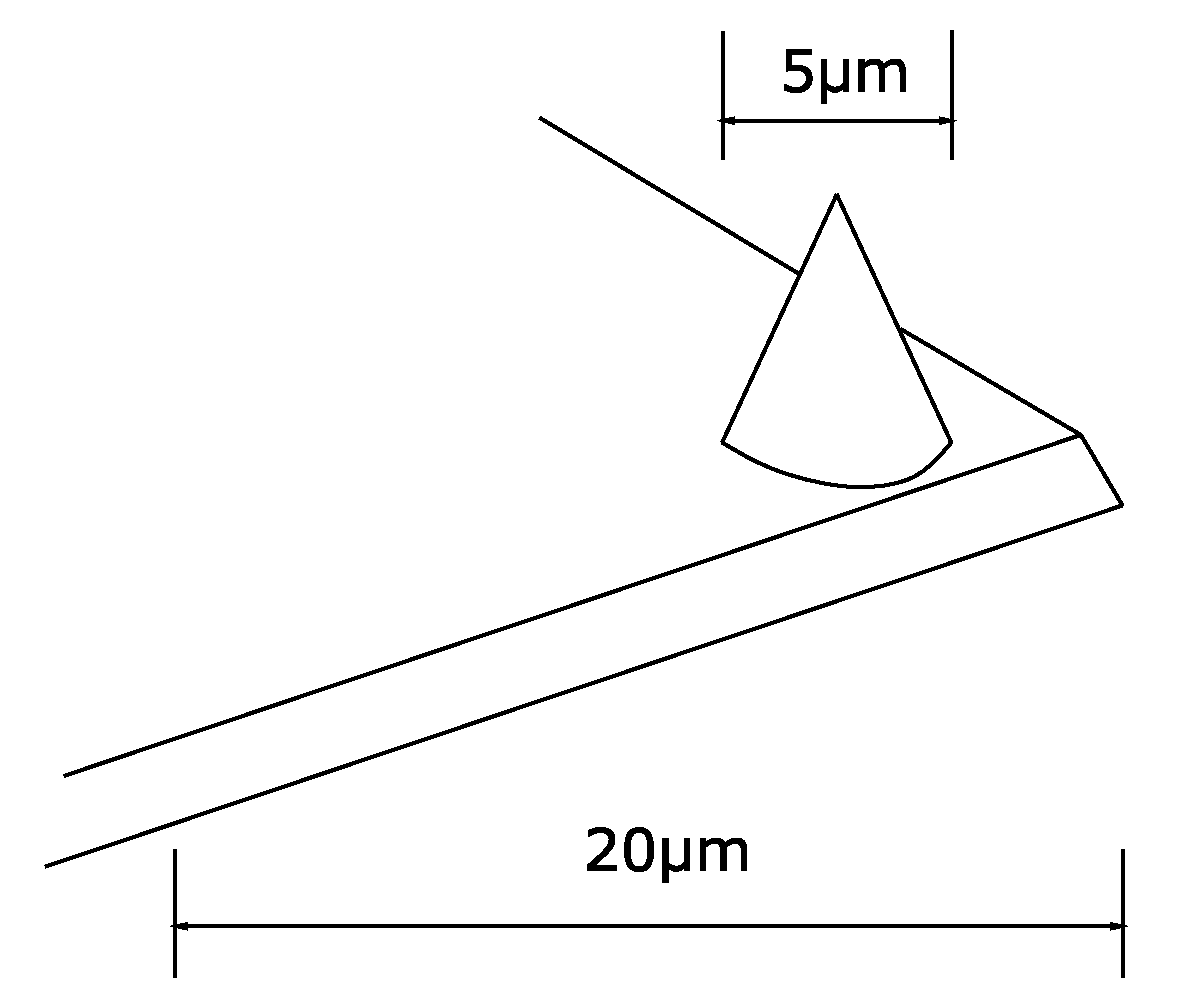
\includegraphics[width=1.2\textwidth]{fig/fig1.pdf}
\caption{力传感器}\label{fig1}
\end{center}
\end{minipage}
\begin{minipage}{0.69\textwidth}
\begin{center}
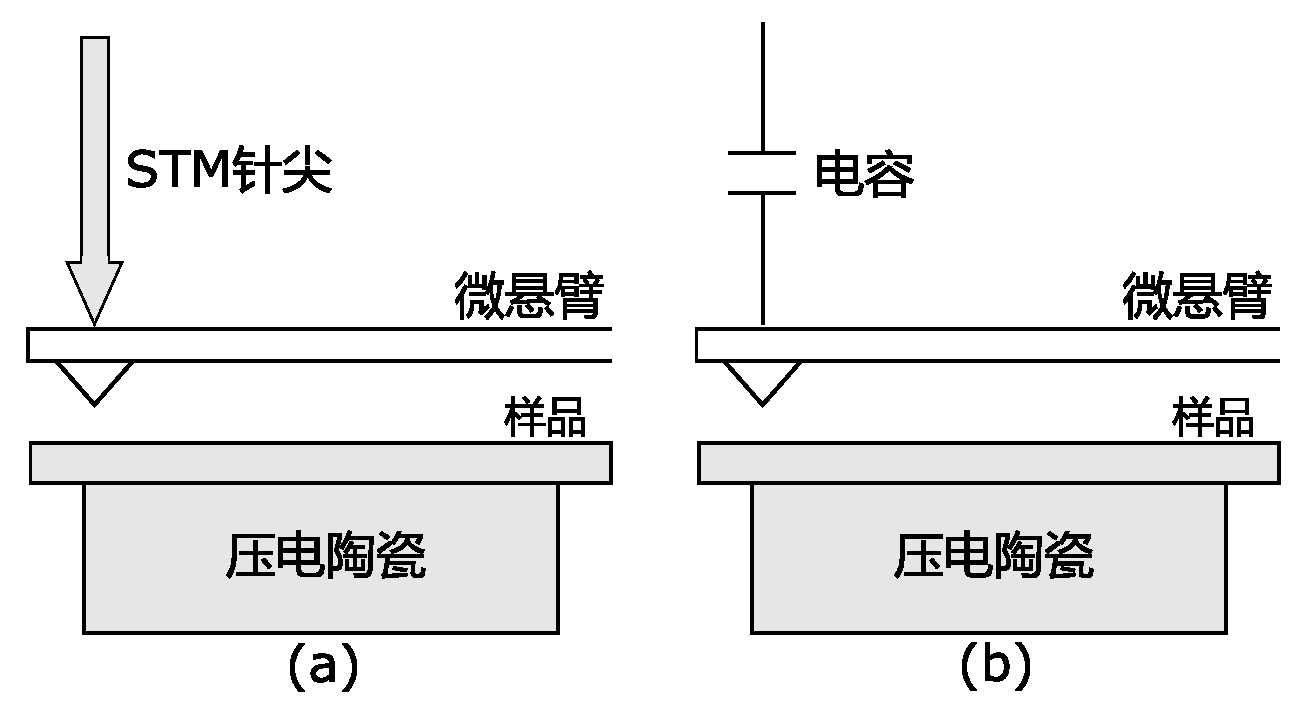
\includegraphics[width=0.85\textwidth]{fig/fig2.pdf}
\caption{微悬臂运动的电学检测法}\label{fig2}
\end{center}
\end{minipage}
\end{figure}

微悬臂运动的检测方法有多种,主要可以分为两大类:电学方法和光学方法。电学方法主要包括隧道电流检测法和电容检测法两种。隧道电流检测法是第一台AFM所采用的方法,它根据隧道电流对电极间距离非常敏感的原理,将SIM用的针尖置于微悬臂的背面作为探测器。如图(\ref{fig2}-a)所示,通过该针尖与微悬臂间产生的隧道电流的变化就可检测由于原子间相互作用力令微悬臂产生的形变。电容法则是通过测量微悬臂与一参考电极间的电容变化来检测微弱力的。如图(\ref{fig2}-b)所示,当微悬臂发生形变时,使它与参考电极间的距离大小发生变化,即电容发生变化,通过测量该电容的变化量就可测量微悬臂的位移。这个方法对于微悬臂针尖与样品的间距无特殊要求。光学法是通过测量激光束在微悬臂背面的反射来测量探针运动的。一种常用的方法如图(\ref{fig3})所示,一束激光经微悬臂背部反射到一个位置灵敏探测器(PSD)上,当微悬臂弯曲时激光束在探测器上的位置将发生移动,PSD本身可测量光点小于$ \SI{1}{nm} $的位移,微悬臂位移的放大倍数为微悬臂至探测器的距离与微悬臂长度之比的两倍。通常这一比例可以做的很大,使得系统可探测针尖在垂直方向上小于$ \SI{0.1}{nm} $的位移。这种方法叫偏转探测法。针尖与样品原子间的作用力十分微弱,数量级小于$ \SI{1e-6}{N} $,它推动微悬臂产生的偏移量也非常小微小,不可能用常规方法直接检测。光点偏转法利用了光杠杆原理将微悬臂的位移放大。
\begin{figure}[!h]
\begin{minipage}{0.48\textwidth}
\begin{center}
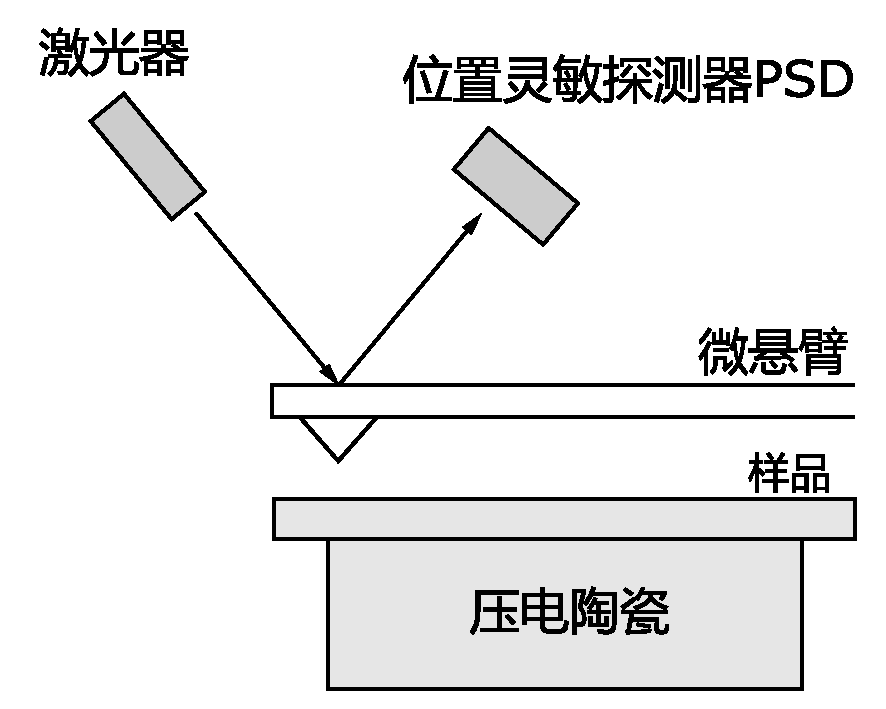
\includegraphics[width=0.9\textwidth]{fig/fig3.pdf}
\caption{微悬臂运动的光学检测法}\label{fig3}
\end{center}
\end{minipage}
\begin{minipage}{0.48\textwidth}
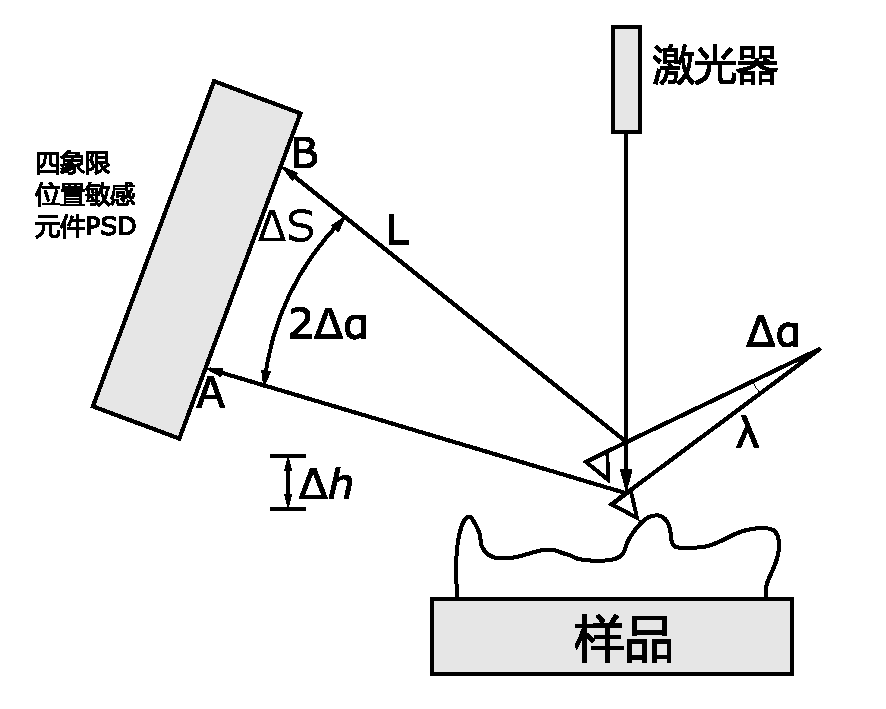
\includegraphics[width=0.9\textwidth]{fig/fig4.pdf}
\caption{光杠杆的位移放大原理}\label{fig4}
\end{minipage}
\end{figure}

如图(\ref{fig4})所示,当激光束聚焦入射到微悬臂外端时,大部分将被反射到QPSD的光敏面上。在起始状态时,反射点位于A,而在原子力状态,样品原子通过针尖推动微悬臂移动$\Delta h$,偏转$\Delta\alpha$角。显然,反射光束将偏转$2\Delta\alpha$角,光点移动到B,位移量$\Delta s$。设微悬臂长$\lambda$,光点接受元件到微悬臂的距离为L,则有
\begin{equation}
\Delta s = L(2\Delta\alpha) = L2\qty(\dfrac{\Delta h}{l}) = \dfrac{2L}{l\Delta h}\label{eq2}
\end{equation}
式(\ref{eq2})表明通过光杠杆的作用,可将针尖的微小位移放大$\dfrac{2L}{\lambda}$倍,在本仪器中取$ L=\SI{10}{cm} $,微悬臂长$\lambda = \SI{200}{\mu m}$,得到
\begin{equation}
\Delta s = \dfrac{2\times 10\times 10^4}{200}\cdot \Delta h = 1000 \Delta h\label{eq3}
\end{equation}
这样,微悬臂的微小位移,反映到光电元件的光敏面上将被放大$ 1000 $倍。如果微悬臂偏转$ \SI{1}{nm} $,光点位移可达$\SI{1}{\mu m}$,这一量级的位移已可被光电元件精确分辨出来。

其它微悬臂位移的光学检测法还有自差法、外差法、干涉法等。与电学方法特别是隧道电流检测法相比,光学法有一些独特的优点:首先,由于激光束束斑的直径为几个微米,这使其反射信号受微悬臂背面粗糙度的影响较小,从而降低了仪器对热漂移的敏感程度;其次,微悬臂背面的污染对光信号影响较小,对隧道电流的影响则相当严重;另外,激光束对微悬臂产生的作用力很小,从而使仪器更加稳定可靠,而且光学法对微悬臂的导电性无要求。
\subsubsection{AFM的工作模式}
当AFM的微悬臂与样品表面原子相互作用时,通常由几种力同时作用于微悬臂,其中最主要的是范德瓦尔斯力。原子力与针尖表面原子间的距离关系曲线如图(\ref{fig5})。利用原子力的性质,我们可以让针尖与样品处于不同的间距,是微悬臂与针尖的工作模式有所不同。AFM有三种不同的工作模式:接触模式(contact mode)、非接触模式(noncontact mode)和共振模式或轻敲模式(tapping mode)。
\begin{enumerate}
\item 接触模式\\
接触模式包括恒力模式(constant force mode)和恒高(constant height mode)。在恒力模式中过反馈线圈调节微悬臂的偏转程度不变,从而保证样品与针尖之间的作用力恒定,当沿x、y方向扫描时,记录z方向上扫描器的移动情况来得到样品的表面轮廓形貌图像。这种模式由于可以通过改变样品的上下高度来调节针尖与样品表面之间的距离,这样样品的高度值较准确,适用于物质的表面分析。在恒高模式中,保持样品与针尖的相对高度不变,直接测量出微悬臂的偏转情况,即扫描器在z方向上的移动情况来获得图像。这种模式对样品高度的变化较为敏感,可实现样品的快速扫描,适用于分子、原子的图像的观察。接触模式的特点是探针与样品表面紧密接触并在表面上滑动。针尖与样品之间的相互作用力是两者相接触原子间的排斥力,约为$\SI{1e-8}{N}\sim\SI{1e-11}{N}$。接触模式通常就是靠这种排斥力来获得稳定、高分辨样品表面形貌图像。但由于针尖在样品表面上滑动及样品表面与针尖的粘附力,可能使得针尖受到损害,样品产生变形,故对不易变形的低弹性样品存在缺点。
\item 非接触模式\\
非接触模式是探针针尖始终不与样品表面接触,在样品表面上方$5\sim\SI{20}{nm}$距离内扫描。针尖与样品之间的距离是通过保持微悬臂共振频率或振幅恒定来控制的。在这种模式中,样品与针尖之间的相互作用力是吸引力——范德华力。由于吸引力小于排斥力,故灵敏度比接触模式高,但分辨率比接触式低。非接触模式不适用于在液体中成像。
\item 轻敲模式\\
在轻敲模式中,通过调制压电陶瓷驱动器使带针尖的微悬臂以某一高频的共振频率和$0.01\sim\SI{1}{nm}$的振幅在z方向上共振,而微悬臂的共振频率可通过氟化橡胶减振器来改变。同时反馈系统通过调整样品与针尖间距来控制微悬臂振幅与相位,记录样品的上下移动情况,即在z方向上扫描器的移动情况来获得图像。由于微悬臂的高频振动,使得针尖与样品之间频繁接触的时间相当短,针尖与样品可以接触,也可以不接触,且有足够的振幅来克服样品与针尖之间的粘附力。因此适用于柔软、易脆和粘附性较强的样品,且不对它们产生破坏。这种模式在高分子聚合物的结构研究和生物大分子的结构研究中应用广泛。
\end{enumerate}
\begin{figure}[H]
\centering
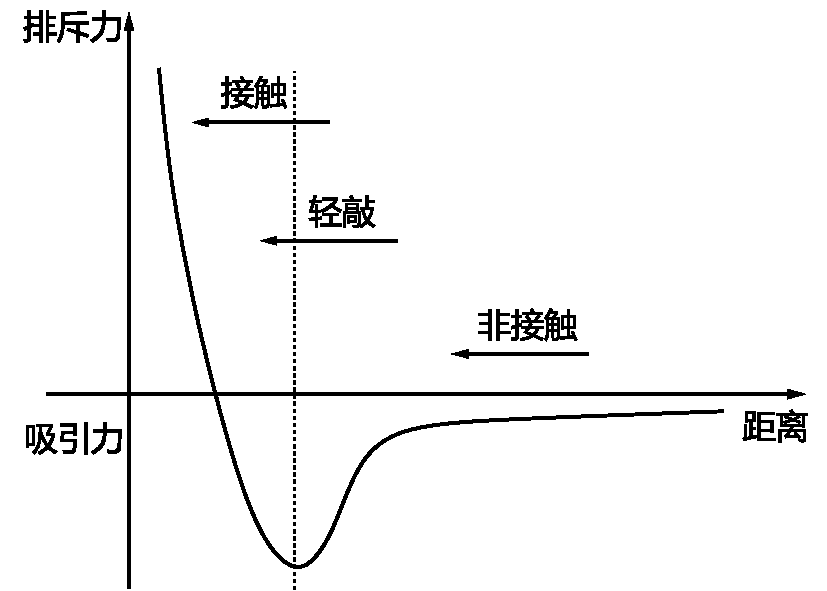
\includegraphics[width=0.8\textwidth]{fig/fig5.pdf}\\
\caption{针尖至样品表面原子间的范德瓦尔斯力}\label{fig5}
\end{figure}
\subsubsection{AFM中针尖与样品之间的作用力}
样品与探针之间的相互作用力主要是针尖最后一个原子和样品表面附近最后一个原子之间的作用力。当探针与样品之间的距离d较大(大于$ \SI{5}{nm} $)时,它们之间的相互作用力表现为范德华力(Van der Waals forces)。可假设针尖是球状的,样品表面是平面的,则范德华力随$\frac{1}{d^2}$变化。如果探针与样品表面相接触或它们之间的间距$ d $小于$ \SI{0.3}{nm} $,则探针与样品之间的力表现为排斥力。这种排斥力与$d^{13}$成反比变化,比范德华力随$ d $的变化大得多。探针与样品之间的相互作用力约为$\num{1e-6}\sim\SI{1e-9}{N}$,在如此小的力作用下,探针可以探测原子,而不损坏样品表面的结构细节。样品与探针的作用力还有其它形式,如当样品与探针在液体介质中相接触时,往往它们的表面由电荷,从而产生静电力;样品与针尖都有可能发生变形,这样样品与针尖之间有形变力;特定磁性材料的样品与探针之间可产生磁力作用;对另一些特定样品和探针,可能样品原子与探针原子之间存在相互的化学作用,而产生化学作用力,但在研究样品与探针之间的作用力的大小时,往往假设样品与探针特定的形状(如平面样品、球面样品),可对样品和探针精心设计与预处理,避免或忽略静电力、形变力、磁力、化学作用力等的影响,而只考虑范德瓦尔斯力和排斥力。
\subsection{AFM的针尖技术}
目前,一般的探针式表面形貌测量仪垂直分辨率已达到$ \SI{0.1}{nm} $,而STM更高,达到$ \SI{0.01}{nm} $,因此足以检测出物质表面的微观形貌。但是,探针针尖曲率半径的大小将直接影响到测量的水平分辨率。针尖技术的发展在AFM中非常重要。其一是发展制得更尖锐的探针,如用电子沉积法制得的探针,其针尖曲率半径在$5\sim\SI{10}{nm}$之间。其二是对探针进行修饰,从而发展起针尖修饰技术。针尖修饰技术在传统探测的物理量(力场、电场、磁场等)的基础上,引入了“化学场”,从而大大地提高和改善了AFM的空间分辨率和物质识别能力。
\subsection{AFM的应用}
AFM可以在真空、超高真空、气体、溶液、电化学环境、常温和低温等环境下工作,在研究时可选择适当的环境。在物理学中,AFM可以用于研究金属和半导体的表面形貌、表面重构、表面电子态及动态过程、超导体表面结构和电子态层状材料中的电荷密度等。从理论上讲,金属的表面结构可由晶体结构推断出,但实际上金属表面很复杂。衍射分析方法已经表明,在许多情况下,表明形成超晶体结构(称为表面重构),可使表面自由能达到最小值。而借助AFM可以方便得到某些金属、半导体地重构图像。AFM可以实现纳米级尺寸和纳米级微弱力的测量。

\section{实验内容}
\begin{enumerate}
%\item 用CCD光学显微镜观察标准光栅(周期为$\SI{100}{\mu m}$)和探针,估算微悬臂有效长度。
\item 安装样品。
\item 进入软件的扫描界面,单击“开始扫描”按钮连续扫描若干次,得到满意图像后单击“捕获图像”按钮以保存图像。
\item 如果要用鼠标选区扫描,必须先按“停止扫描”按钮再用鼠标选区。否则可能损坏探针。
\item 先按“停止扫描”按钮,再退出扫描界面。
\item 退出样品。
\item 数据处理:再软件的图像处理界面完善图像,标注尺寸、记录相应的粗糙度统计结果、做三维效果图。
\item 打印图像。
\end{enumerate}

\section{实验数据}
\subsection{厚样品}
图\ref{fig6}, \ref{fig7}, \ref{fig8}分别是厚样品的扫描结果,3D显示图和傅里叶变换图。观察发现,厚样品具有明显的周期性结构。在二维傅里叶变换图中,选择1:8的放大率以更好的发现频率峰值。找到频率峰值所对应的X周期、Y周期、R周期分别是3750nm、2500nm和2000nm。
\begin{figure}[htbp]
\centering
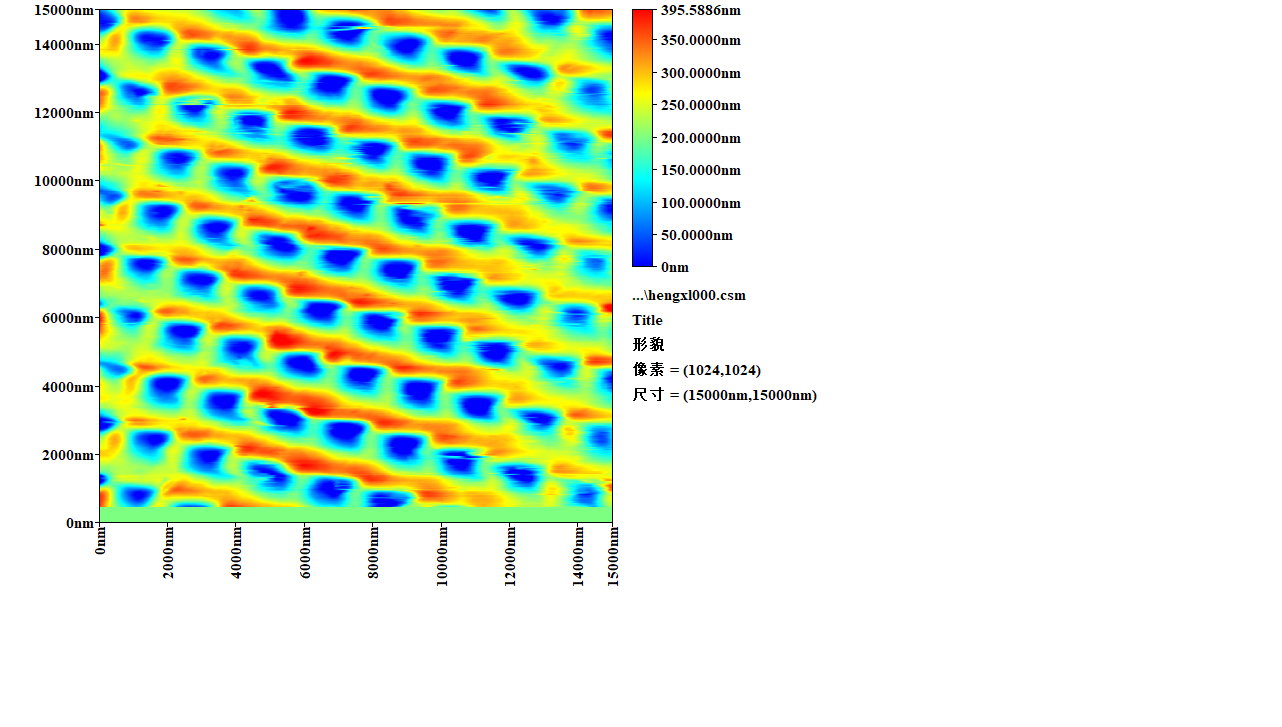
\includegraphics[width=0.6\textwidth]{data/0/hengxl000C.png}\\
\caption{扫描结果}\label{fig6}
\end{figure}

\begin{figure}[htbp]
\centering
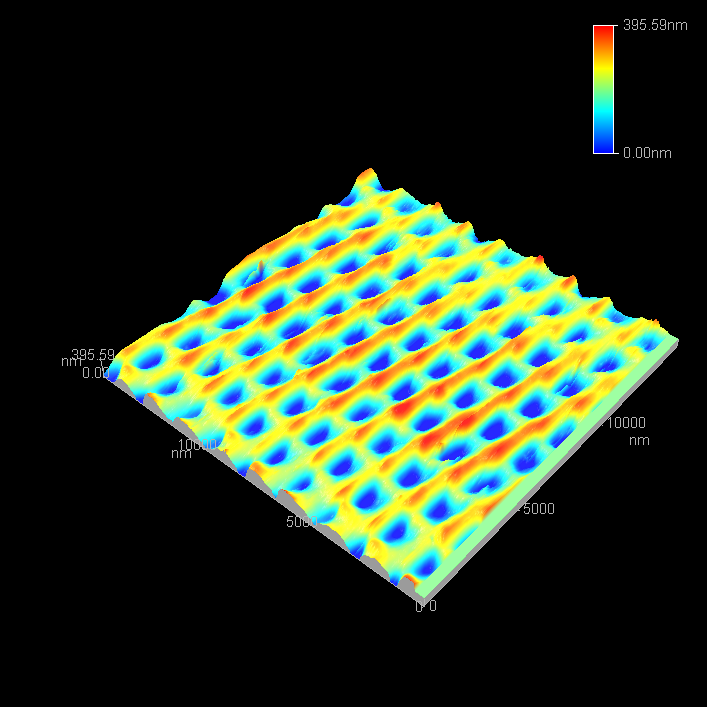
\includegraphics[width=0.6\textwidth]{data/0/hengxl0003D.png}\\
\caption{3D显示}\label{fig7}
\end{figure}

\begin{figure}[htbp]
\centering
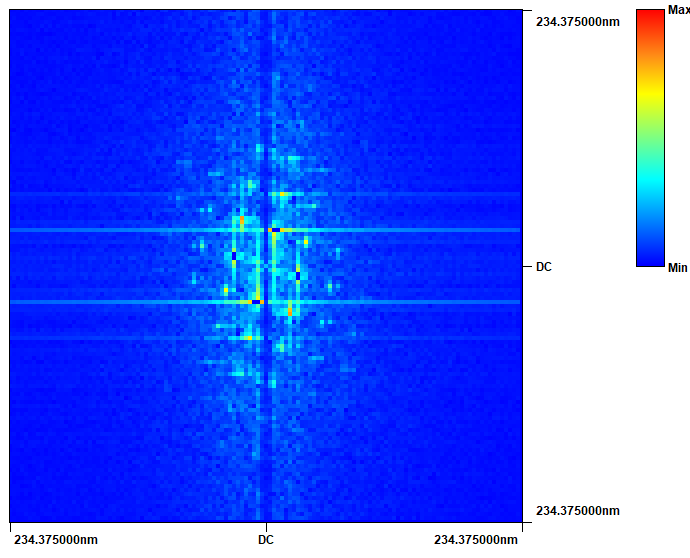
\includegraphics[width=0.6\textwidth]{data/0/hengxl000_FFT.png}\\
\caption{傅里叶变换图}\label{fig8}
\end{figure}

\subsection{薄样品}
图\ref{fig9}是薄样品的扫描结果和粗糙程度分析,其中比较重要的信息有以下几点。
\begin{enumerate}
	\item 样品的极差约为7nm,但平均高度只有0.7nm,说明样品整体高度较低。
	\item 样品的均方根为1.04nm,说明样品的粗糙起伏程度不大。
\end{enumerate}
\begin{figure}[htbp]
\centering
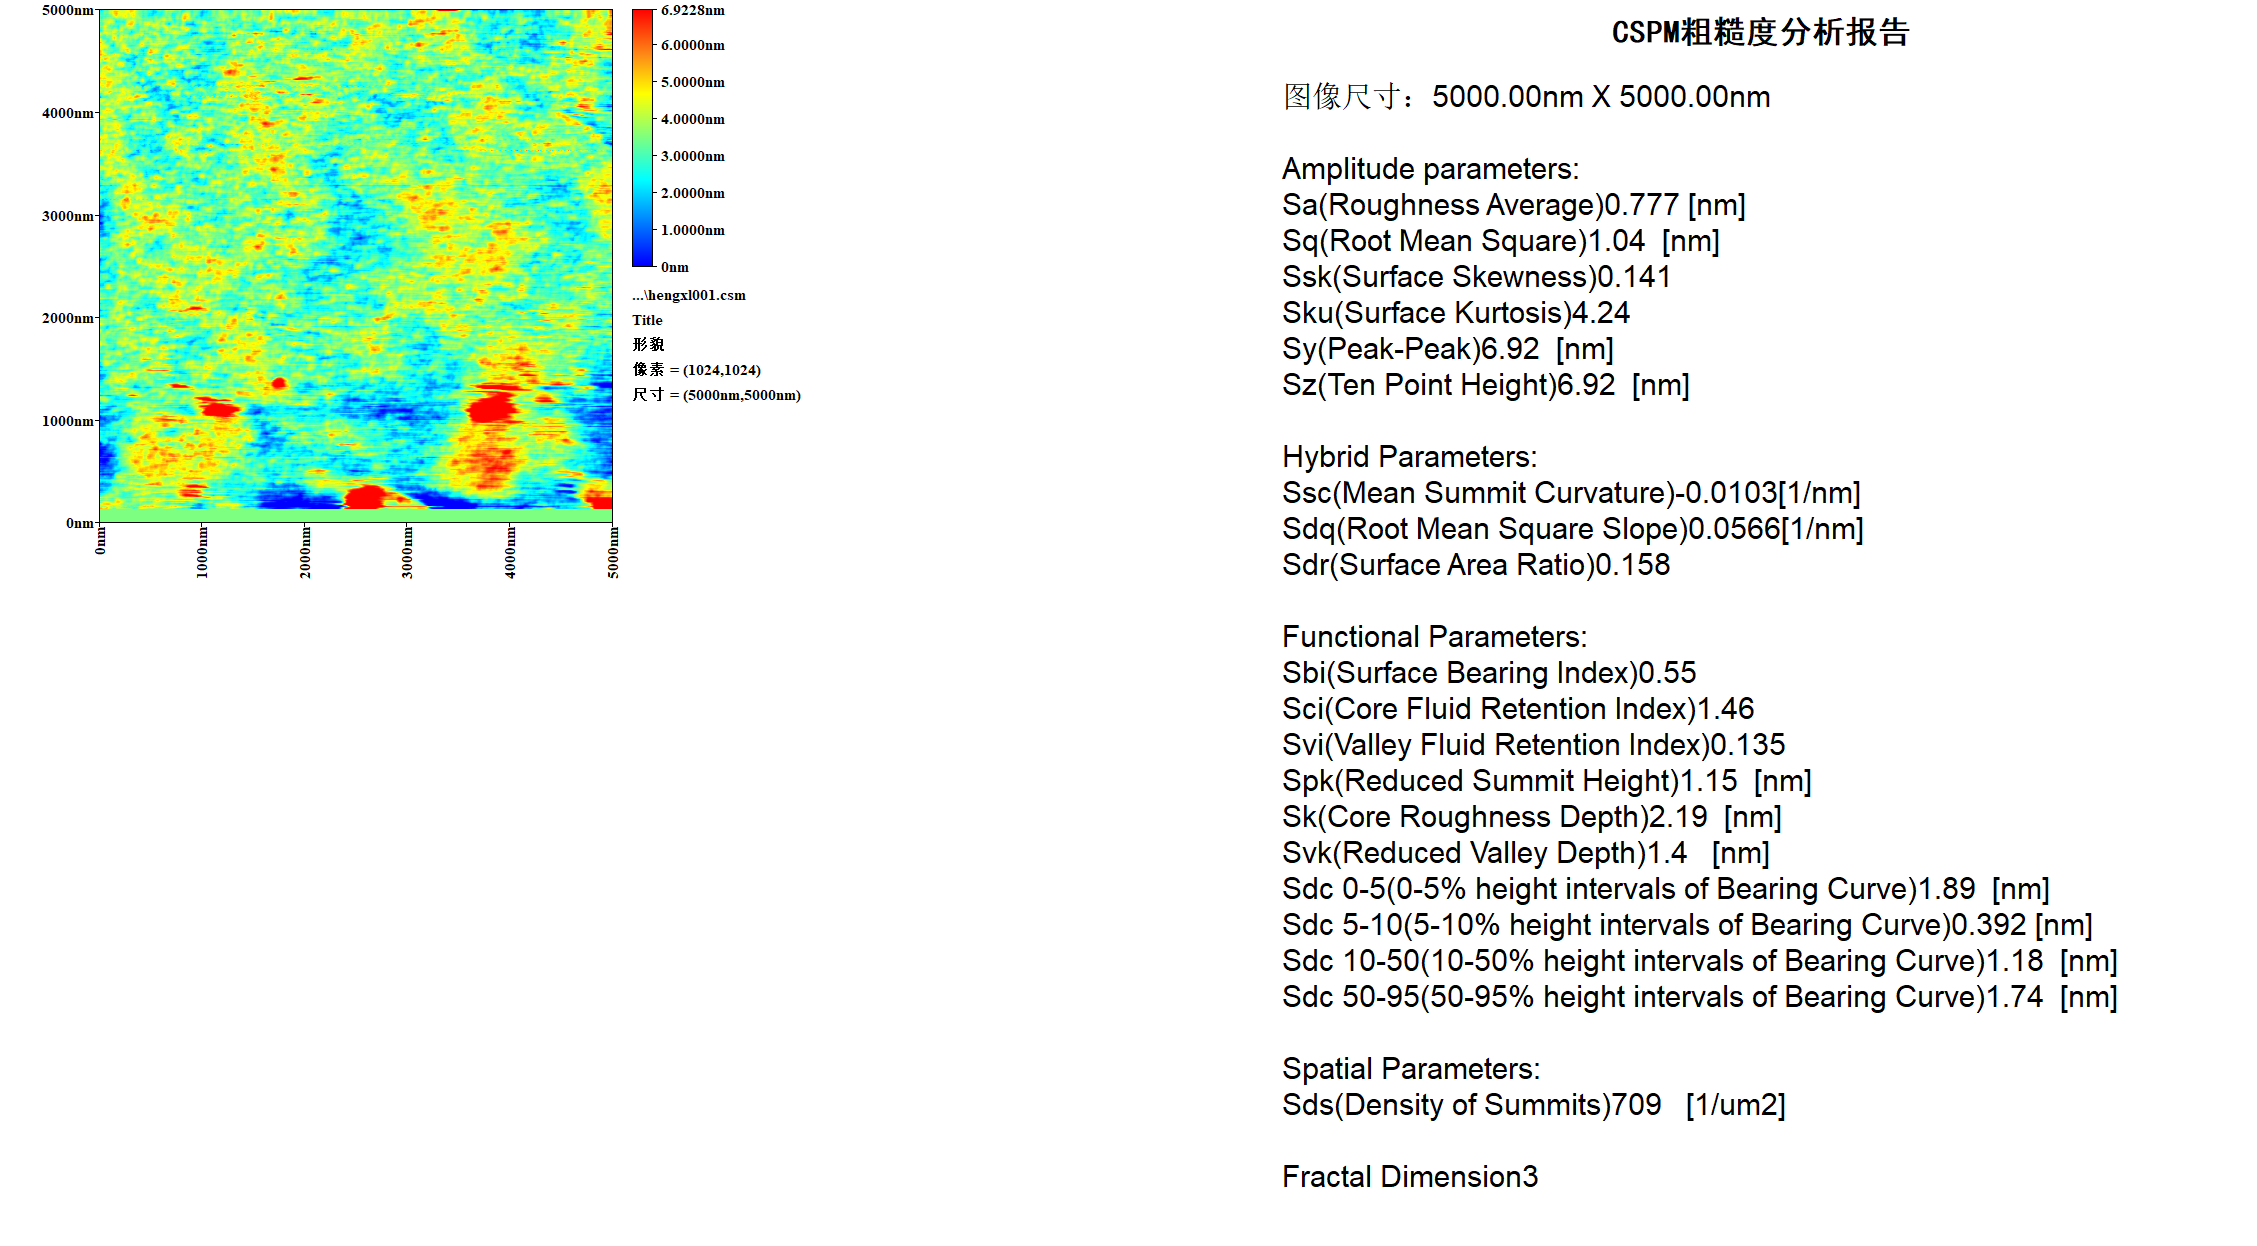
\includegraphics[width=0.8\textwidth]{data/1/hengxl001_ROU.png}\\
\caption{扫描结果和粗糙程度分析}\label{fig9}
\end{figure}

\section{思考题}
\subsection*{AFM探测到的原子力的由哪两种主要成分组成?}
原子之间的Van de Waals相互作用,表现为吸引力;相近原子之间电子云的相互作用,表现为排斥力。
\subsection*{怎样使用AFM和CCD光学显微镜,才能较好的保护探针?}
\begin{enumerate}
	\item 在移动探头和底座时需注意轻拿轻放;
	\item 在放置样品前要注意探针的位置,如果探针位置太深应提前退针;
	\item 测量完毕后应及时退针,以免原子力持续作用在探针上。
\end{enumerate}
\subsection*{原子力显微镜有哪些应用?}
原子力显微镜可以克服传统光学显微镜的分辨率限制,精细地扫描材料表面,获得材料表面形貌、粗糙结构等信息,这对研究表面材料、二维材料等都有很大的意义。
\subsection*{与传统的光学显微镜,电子显微镜相比,扫描探针显微镜的分辨本领主要受什么限制?}
主要受探针的尺寸,探针的材料限制。也与移动探针的电机灵敏度有关。
\subsection*{要对悬臂的弯曲量进行精确测量,除了在AFM中使用光杠杆这个方法外,还有哪些方法可以达到相同数量级的测量精度?}
在STM显微镜中,为了测量悬臂的弯曲量,运用了量子隧穿效应。根据隧穿电流的大小确定悬臂的弯曲量。

\nocite{jiaocai}
\bibliography{ref}
\end{document}